%Critique.tex
%Par Guillaume Lahaie
%LAHG04077707
%
%Critique du SRS Gestion de centre sportif fourni dans le cours. J'utilise un gabarit de tex pour l'écriture

%%%%%%%%%%%%%%%%%%%%%%%%%%%%%%%%%%%%%%%%%
% Simple Sectioned Essay Template
% LaTeX Template
%
% This template has been downloaded from:
% http://www.latextemplates.com
%
% Note:
% The \lipsum[#] commands throughout this template generate dummy text
% to fill the template out. These commands should all be removed when 
% writing essay content.
%
%%%%%%%%%%%%%%%%%%%%%%%%%%%%%%%%%%%%%%%%%

%----------------------------------------------------------------------------------------
%	PACKAGES AND OTHER DOCUMENT CONFIGURATIONS
%----------------------------------------------------------------------------------------

\documentclass[11pt]{article} % Default font size is 12pt, it can be changed here
\renewcommand{\familydefault}{\rmdefault}
\renewcommand{\thesubsection}{\alph{subsection}}


%Pour l'encodage avec accents
\usepackage[utf8]{inputenc}

\usepackage{helvet}
\renewcommand{\familydefault}{\sfdefault}

\usepackage{afterpage}
\usepackage{appendix}
\usepackage{graphicx} % Required for including pictures
\usepackage{listings}

\usepackage[left=2.2cm,top=2.2cm,right=2.2cm,bottom=2.2cm,nohead]{geometry} % Required to change the page size to A4
\geometry{letterpaper} % Set the page size to be A4 as opposed to the default US Letter



\usepackage{float} % Allows putting an [H] in \begin{figure} to specify the exact location of the figure
\usepackage{wrapfig} % Allows in-line images such as the example fish picture

\usepackage{lipsum} % Used for inserting dummy 'Lorem ipsum' text into the template


\linespread{1.2} % Line spacing

%\setlength\parindent{0pt} % Uncomment to remove all indentation from paragraphs

\graphicspath{{./Pictures/}} % Specifies the directory where pictures are stored
\usepackage[french,english]{babel}

%Comportement d'un paragraphe
\setlength{\parskip}{\baselineskip}%
\setlength{\parindent}{0pt}%

%Widows/orphans
\widowpenalty10000
\clubpenalty10000

\usepackage[hidelinks]{hyperref}

%Meta-info
\title{INF4500 - devoir 1}
\author{Guillaume Lahaie}
\date{Remise: 1er novembre 2013}

\hypersetup{
  pdftitle={INF4500 - devoir 1},
  pdfauthor={Guillaume Lahaie}
}

\newcommand\blankpage{%
  \null
  \thispagestyle{empty}%
  \addtocounter{page}{-1}%
  \newpage}

\begin{document}
\selectlanguage{french}

%----------------------------------------------------------------------------------------
%	TITLE PAGE
%----------------------------------------------------------------------------------------

\begin{titlepage}

\newcommand{\HRule}{\rule{\linewidth}{0.5mm}} % Defines a new command for the horizontal lines, change thickness here

\center % Center everything on the page

\textsc{\LARGE Université du Québec à Montréal}\\[1.5cm] % Name of your university/college
\textsc{\Large INF4500}\\[0.5cm] % Major heading such as course name

\HRule \\[1.5cm]
{ \huge \bfseries Devoir 1}\\[0.4cm] % Title of your document
\HRule \\[1.5cm]

\begin{minipage}{0.4\textwidth}
\begin{flushleft} \large
\emph{Par:}\\
Guillaume Lahaie \\ LAHG04077707 % Your name
\end{flushleft}
\end{minipage}
~
\begin{minipage}{0.4\textwidth}
\begin{flushright} \large
\emph{Remis à:} \\
Abdoulaye Baniré Diallo % Supervisor's Name
\end{flushright}
\end{minipage}\\[4cm]

{\large \emph{Date de remise:} \\ Le 1\textsuperscript{er} novembre 2013}\\[3cm] % Date, change the \today to a set date if you want to be precise

%\includegraphics{Logo}\\[1cm] % Include a department/university logo - this will require the graphicx package

\vfill % Fill the rest of the page with whitespace

\end{titlepage}
\blankpage

%----------------------------------------------------------------------------------------
%	TABLE OF CONTENTS
%----------------------------------------------------------------------------------------

\tableofcontents % Include a table of contents

\newpage % Begins the essay on a new page instead of on the same page as the table of contents 

%----------------------------------------------------------------------------------------
% SECTIONS DU DOCUMENT
%----------------------------------------------------------------------------------------

\section{Question 1} % Major section

\subsection[Description du gène ALS2]{Donnez une description sommaire de ce locus chez l'humain. Celle-ci devra 
minimalement contenir les informations suivantes: sa location précise, sa taille, son rôle,
et toutes autres descriptions que vous jugerez pertinente.}

J'ai consulté deux sources pour obtenir des informations sur la location du gène ALS2 de l'humain. La première source,
afin d'identifier la location du locus, était le UCSS genome browser. La recherche a été effectuée sur la version GRCh37/hg19
du génome humain. Comme on peut le voir sur l'image en annexe \ref{1},le
gène ALS2 est sur le brin q, c'est-à-dire qu'il est sur le brin complémentaire, donc il est orienté 3` $->$ 5`.

Le locus du gène est situé sur le chromosome, à la position 2q33.1. La position précise du gène est chr2:202,564,986-202,645,895.
Sa taille est donc 80 910 pairs de nucléotides. 

Afin de vérifier la validité de l'information, j'ai effectué la même recherche dans la base de données du
\emph{National Center for Biotechnology Information} (NCBI). J'ai effectué une recherche dans la base de données des gènes,
j'insère en annexe \ref{2}  une image de la région du chromosome 2 où se situe le gène. On retrouve les mêmes informations
à propos du gène ALS2 sur NCBI: il est situé à la location 2q33.1, plus précisemment sur le chromosome 2:202564986..202645895, 
il a donc la même taille de 80 910 pairs de nucléotides.

NCBI donne un sommaire de la fonction du gène ALS2, toutefois cette description ne donne pas une description pratique.
Afin d'avoir une meilleure idée de la fonction du gène ALS2, j'ai effectué une recherche sur \emph{Genetics Home Reference} (GHR).
Le gène ALS2 (amyotrophic lateral sclerosis 2 (juvenile)) a comme fonction la production de la protéine alsin. Cette protéine
semble avoir plusieurs rôles, entre autres l'activation de protéines de la famille des GTPases, qui joue un rôle important dans
la division cellulaire, la différentiation.

Selon GHR, au moins huit mutations du gène ALS2 causent la Sclérose latérale amyotropique, aussi connue sous le nom de la
maladie de Lou Gherig. Toutefois, seulement 5 à 10\% des cas de cette maladie serait de cause génétique. Afin de trouver
d'autres caractéristiques de ce gène, j'ai téléchargé le fichier genbank de la région particulière du chromosome 2.
J'ai ensuite écrit un script en biopython afin de calculer la distribution des nucléotides de ce locus (annexe \ref{3}). Voici les résultats:
\begin{center}
\begin{tabular}{|c|c|c|}
 \hline
 Nucléotides & Compte & Pourcentage \\
 \hline
 A & 23361 & 28.87\% \\
 \hline
  C & 15070 & 18.62\% \\
 \hline
  G & 15717 & 19.43\% \\
 \hline
  T & 26762 & 33.08\% \\
 \hline
  Total & 80910 & 100\% \\
 \hline
\end{tabular}
\end{center}




%----------------------------------------------------------------------------------------
% SECTIONS DU DOCUMENT
%----------------------------------------------------------------------------------------
 
\section{Éric Fournier (chef d'équipe)}

{\LARGE Note: 100 / 100}
 
Rien à redire sur son travail. A pris en charge le SRS au début de la session, et ensuite a
fait une bonne partie du prototype, en s'occupant aussi des suivis hebdomadaires, et aussi
faire le suivi avec chaque membre.
 
%----------------------------------------------------------------------------------------
% SECTION VALIDATION
%----------------------------------------------------------------------------------------
 
\section{Maxime Girard}

{\LARGE Note: 90 / 100}

Il s'est occupé d'une des parties importantes du prototype surtout. Je pense qu'il aurait pu nous donner un
peu plus de feedback sur ses progrès, généralement j'ai l'impression que c'était surtout ça avance, ça avance pas, 
pas plus de détail que ça.


%----------------------------------------------------------------------------------------
% CONCLUSION
%----------------------------------------------------------------------------------------
 
\section{Marco Gagliano} 
 
{\LARGE Note: 80 / 100}

Malgré qu'il ait participé à toutes les réunions et qu'il ait faite une grande partie du protoype, c'était
difficile de prévoir quand le travail serait fait. Il y a eu quelques semaines où il n'a rien fait. Au moins,
à une reprise, il nous en a averti à l'avance. À certains moments, il disait n'avoir plus le temps
de faire certains parties du projet, mais finalement il les faisait, c'était donc un peu difficile
d'organiser les tâches.

J'ai trouvé aussi qu'on avait des attentes différentes à propos du projet. Il a dit à quelques reprises
que ce n'était pas nécessaire de trop se forcer, que si on avait un B+ pour le cours c'était assez. J'avais
une opinion différente.



\begingroup
\renewcommand{\appendix}{%
    \renewcommand{\thesubsection}{\arabic{subsection}}
}

\appendix
\section{Annexes}
\subsection{Image du locus du gène ALS2 chez l'homo sapien du UCSC genome browser}\label{1}
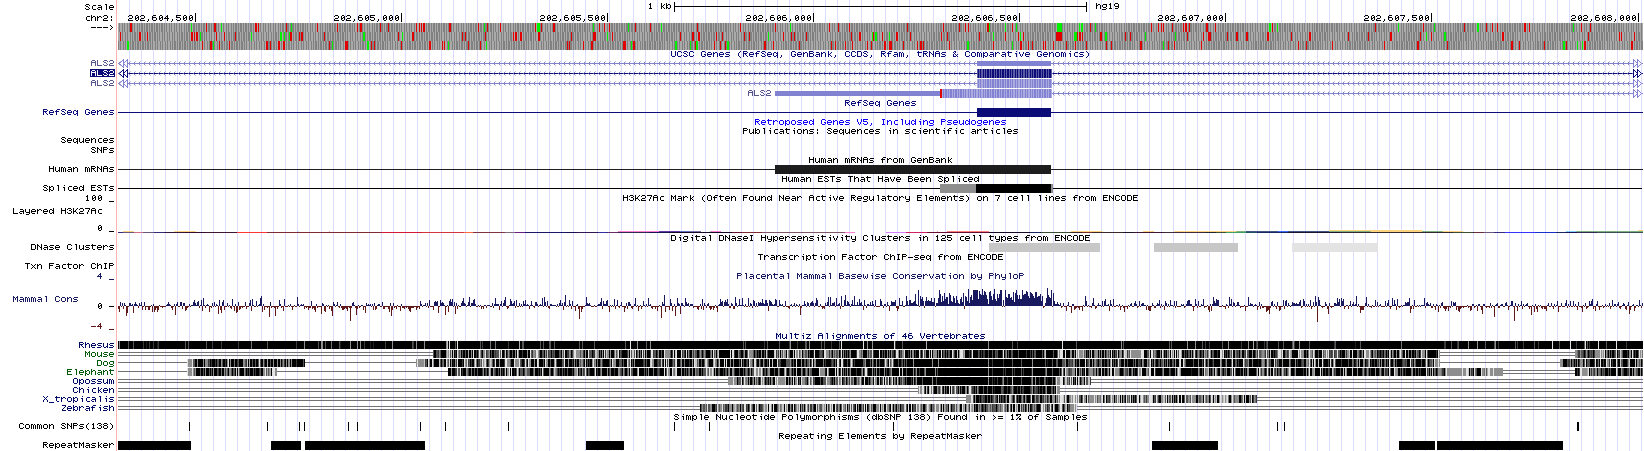
\includegraphics[width=\linewidth]{annexes/annexe1_ucsc.png}

\subsection{Image du locus du gène ALS2 chez l'homo sapien de NCBI}\label{2}
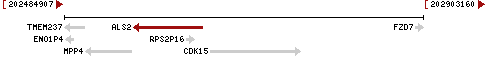
\includegraphics{annexes/annexe1_ncbi_als2.png}

\subsection{Script biopython de calcul des fréquences nucléotidiques}\label{3}
\begin{lstlisting}[frame=single,numbers=left,language=Python]
# -* coding:utf-8 *-#
from Bio import SeqIO
from Bio.SeqRecord import SeqRecord
handle = open("NC_000002_202564986-202645895.gb", "r")
seq_record = SeqIO.parse(handle, 'gb')
for seq in seq_record:
    dist_a = seq.seq.count("A")
    dist_c = seq.seq.count("C")
    dist_g = seq.seq.count("G")
    dist_t = seq.seq.count("T")
    print "A:  count: " + str(dist_a) + " % = " + \
        str(float(dist_a)/len(seq)*100)
    print "C:  count: " + str(dist_c) + " % = " + \
        str(float(dist_c)/len(seq)*100)
    print "G:  count: " + str(dist_g) + " % = " + \
        str(float(dist_g)/len(seq)*100)
    print "T:  count: " + str(dist_t) + " % = " + \
        str(float(dist_t)/len(seq)*100)
    print "total = " + str(dist_a+dist_c+dist_g+dist_t)
\end{lstlisting}

\endgroup

%
%Bibiographie
%
\begin{thebibliography}{99}
\bibitem{UCSC genome browser}
    Kent WJ, Sugnet CW, Furey TS, Roskin KM, Pringle TH, Zahler AM, Haussler D. The human genome browser at UCSC. 
    \emph{Genome Res.} 2002 Jun;12(6):996-1006. 
\bibitem{Genetics Home Reference}
    National Library of Medicine (US). Genetics Home Reference [Internet]. Bethesda (MD): The Library; 2013 Oct 26. ALS2; [reviewed 2012 Aug; cited 2013 Oct 26]. Available from: http://ghr.nlm.nih.gov/gene/ALS2
\bibitem{Wikipedia-SAL}
  Sclérose latérale amyotrophique. In Wikipedia. Retrieved October 26, 2013, from http://fr.wikipedia.org/wiki/Scl%C3%A9rose_lat%C3%A9rale_amyotrophique

\end{thebibliography}
\end{document}